\section{Discussion}
\label{sec:results}

\subsection{Impact of label noise on feature transferability}


%%%%%%%% FIGURE Number of training categories
\begin{figure}[t]
\centering
   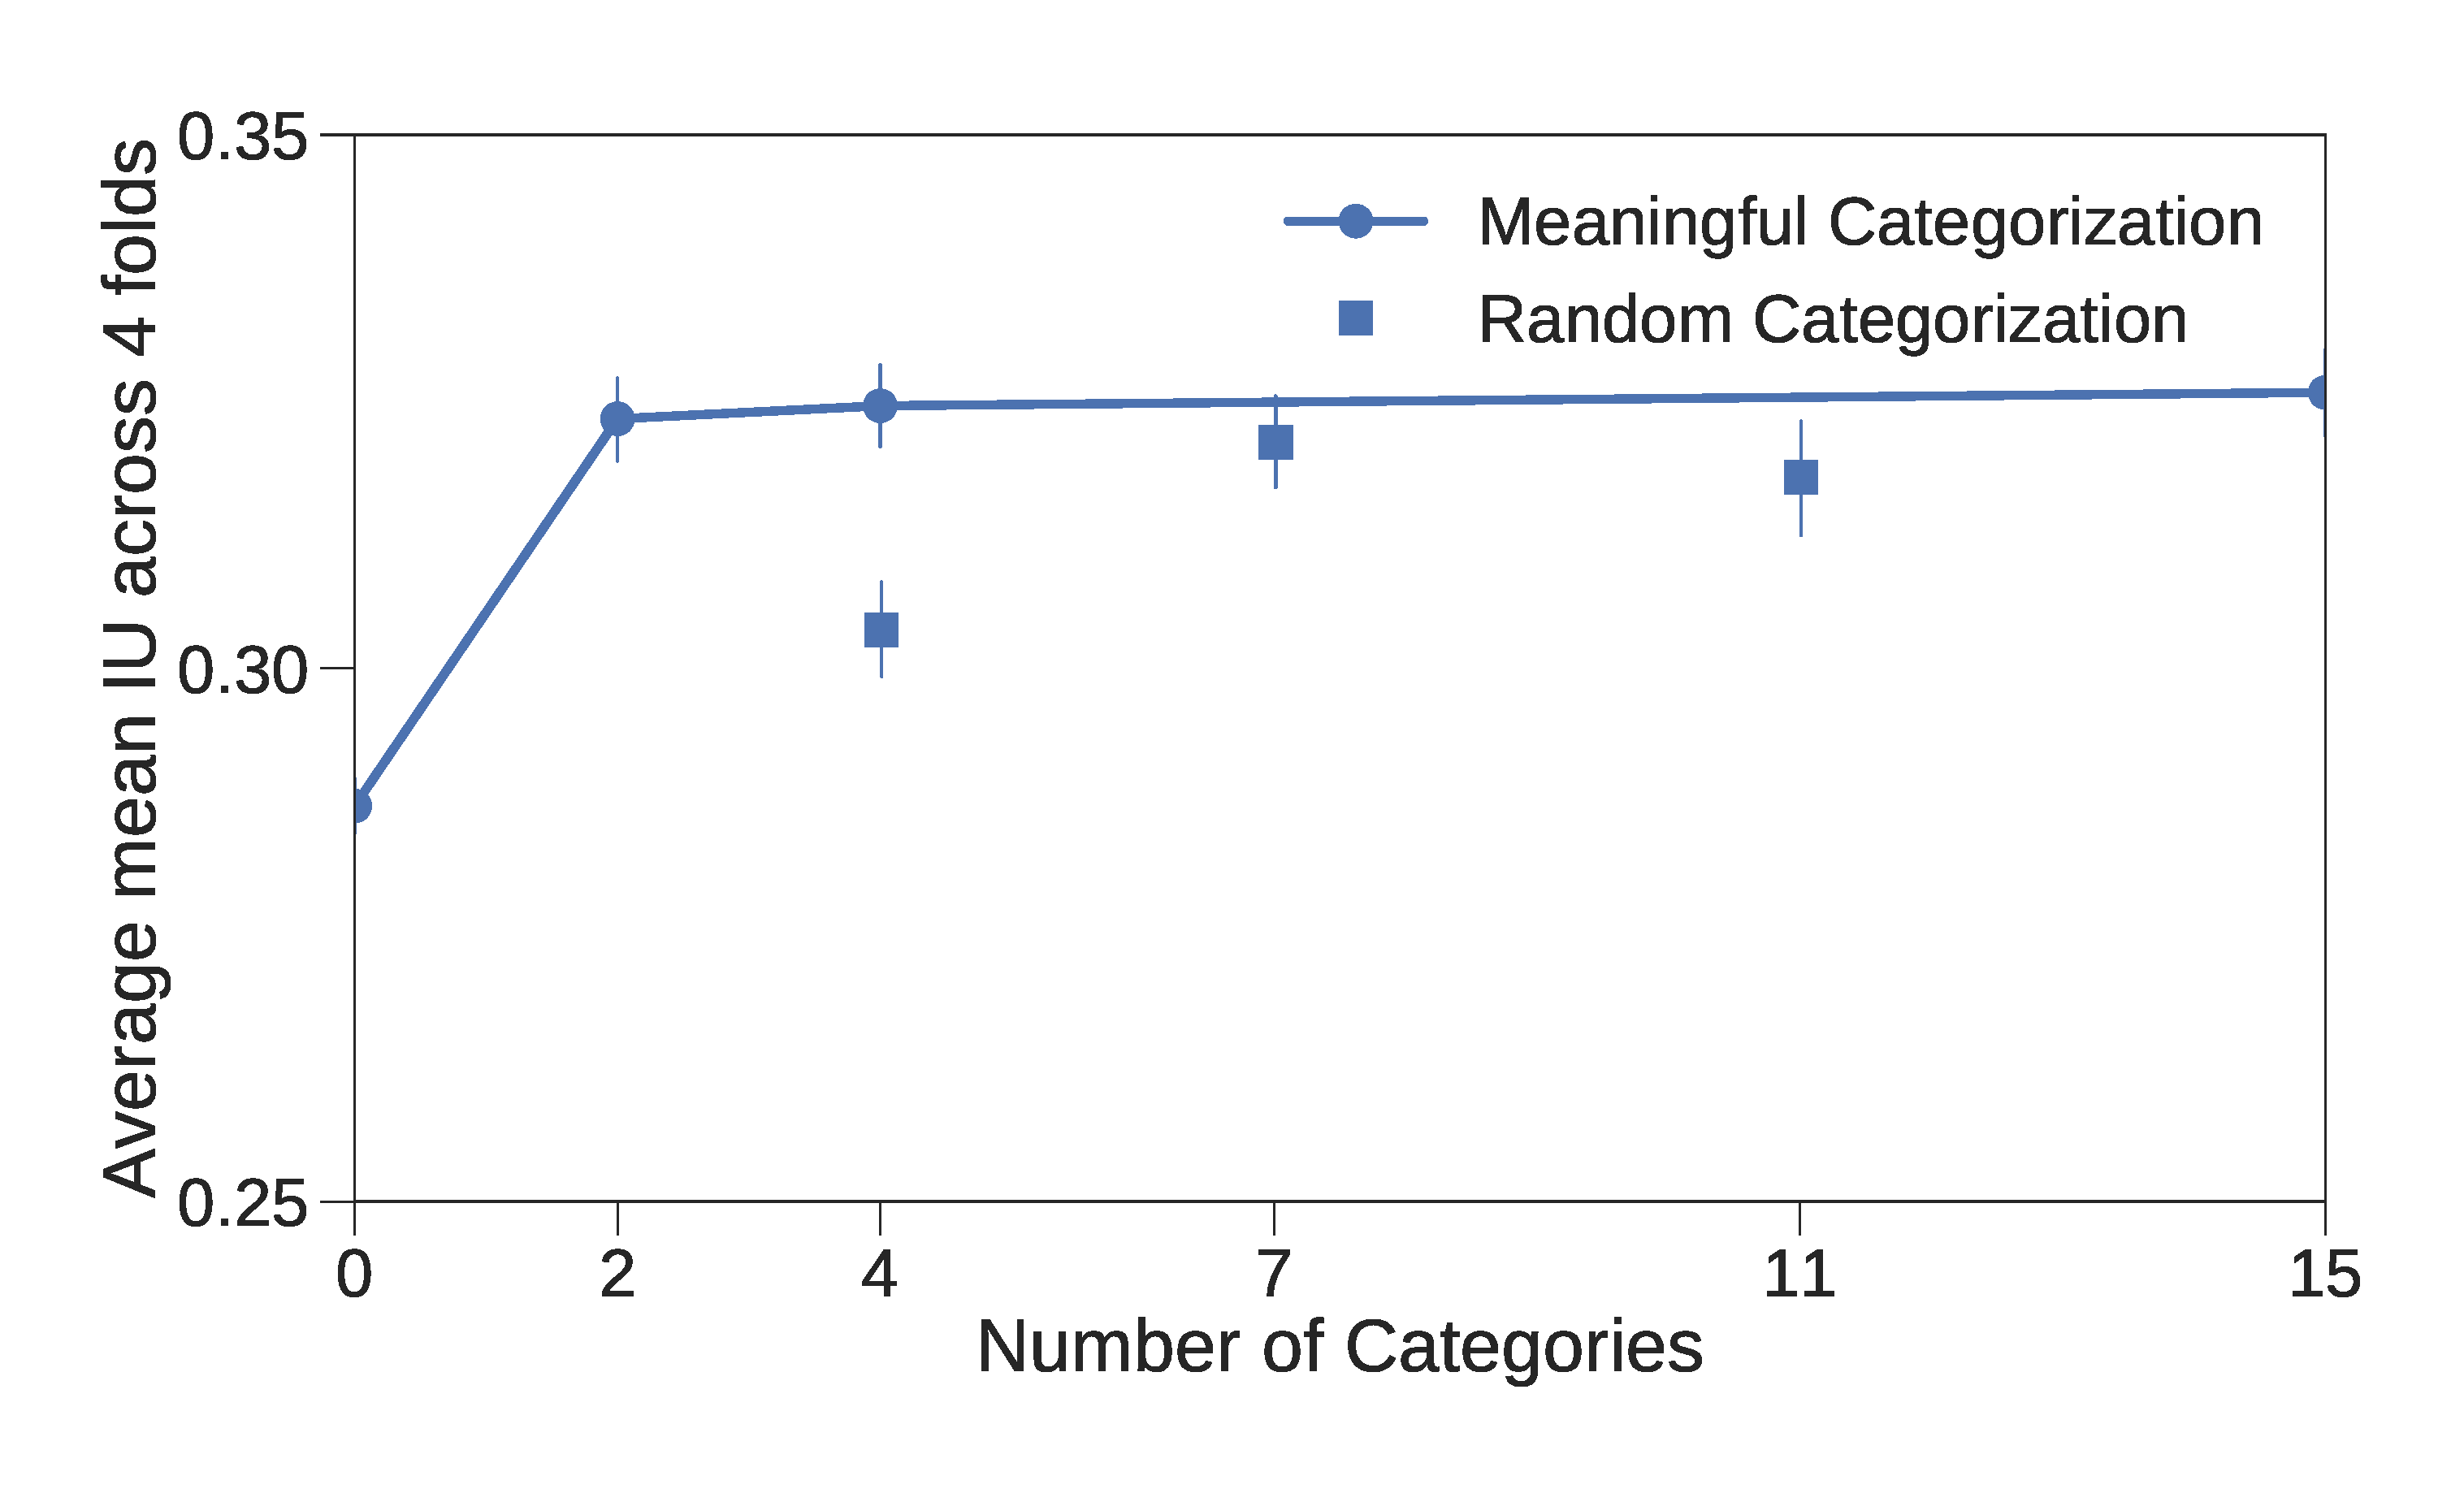
\includegraphics[width=1.\linewidth]{img/num_classes.eps}
\caption{
The influence of number of categories in the pre-training dataset on performance of fine-tuned models.
Varying the number of categories while pre-training the representation and the pre-trained weights were fine-tuned to segment 5 categories from the PASCAL VOC2011 dataset
}
\label{fig:categories}
\end{figure}

% %%%%%%%% FIGURE First-layer feature visualization
% \begin{figure}[t]
% \centering
% \fbox{\rule{0pt}{2in} \rule{0.9\linewidth}{0pt}}
%   %  \includegraphics[width=0.95\linewidth]{img/}
% \caption{Visualization of first-layer features from different pre-trained models.}
% \label{fig:features}
% \end{figure}

\begin{itemize}
  \item
  \item Pixel independent noise assumption
  \item Logistic loss optimize accuracy, not mean IU
\end{itemize}
